\chapter{Proposed methology}
\label{chapter:methods}

%You have now stated your problem, and you are ready to do something
%about it!  \emph{How} are you going to do that? What methods do you
%use?  You also need to review existing literature to justify your
%choices, meaning that why you have chosen the method to be applied in
%your work.

In this chapter we will finally propose a methology to try to solve the problems introduced in the previous chapter.
We will be reviewing, what we will be doing in the implementation part of this thesis and analyze the information that we have seen to this point.
Finally, we will look how we will evaluate the end-product and how is it better or worse than other alternatives.

As stated in the chapter about requirements, there are multiple points that can hinder the development of big data pipeline for stock data analysis for novice data scientist.
In this chapter we will introduce our method which can help novice data scientist to build more efficiently big data pipelines for stock analysis.

We will start by introducing the overview of the method and the steps that it consist of.
We then examine each step giving our reasoning why to do it like depicted in the step.
Finally, we end the chapter by defining how are we going to test this method in the following chapters.

\section{Overview}

Our method to build novice friendly big data pipelines for stock market analysis is divided into 5 steps, which are mostly focused on planning the pipeline.
The steps are the following:

\begin{enumerate}
    \item Pick a data source for stock data
    \item Pick either Scala or Python as main programming language
    \item Pick technology for each part of pipeline
    \item Implement the architecture using Docker and Docker Compose
    \item Share the pipeline (if possible) and start developing
\end{enumerate}

The process is quite simple and each of the steps are explained more throughly in the following sections with some examples, but here we examine the basic reasoning behind each step.
Every process starts with picking a data source for stock data as the format of the data specifies what are the requirements for ingestion of the system and as such is a pretty trivial step.
The main problem with data sources is the low amount of relevant data sources which is why we have listed some in the following section.

We recommend picking either Scala or Python as the main programming language and using it as much as possible in the pipeline.
Both have the needed libraries that can be used to analyse stock data with machine learning methods while taking into account the big data aspect.
Choosing one reduces the complexity of the pipeline and because both have a very versatile supply of libraries choosing one over the other does not reduce the options of the user.
Choosing Scala, however, might restrict the amount of available information online as Python has very active community \cite{giang}.

For selecting technologies we unfortunately cannot give any universal instructions.
As said in the previous section, there are too many integrations to consider on how each component works with another to ensure that the system is optimal for each use case.
However, we have provided one example on the technology selection.
The last two steps are more thoroughly reasoned in the Section 4.1.4.

\subsection{Data source}

Our first step in the methology has to do with picking up the data source and is directly linked to our requirement R1.
Of course, if the user of this method already has a data source for stock data then we definitely recommend skipping this step and moving to the next one. 
As most of the data sources concerning stock data are closed and heavily priced we have gathered here the most promising data sources that novice data scientist could use as their starting point.
These are picked based on their pricing and the amount of public information these services provide about themselves.
A list of this kind of services is presented in Table 4.1.

\begin{table}[! htbp]\centering 
    \caption{Stock data sources}
    \begin{threeparttable}
        \begin{tabular}{|p{2cm}|p{2.5cm}|l|p{2cm}|p{3cm}|} 
        \hline
        & Type of data & Minimum Price & Data Structure & Restrictions \\ \hline
        IEX \cite{iex}& Intraday and Historical (15 years) & 0\$/month & JSON & 500k datapoints/month \\ \hline
        Alpha Vantage \cite{alphavantage}  & Intraday and Historical (20+ years)& 0\$/month & JSON/CSV & 5 requests/min and 500/day\\ \hline
        World Trading Data \cite{worldtradingdata} & Intraday and Historical (from 1980) & 0\$/month & JSON/CSV & 5 symbols/request, 250 request/day and 25 intraday requests/day\\ \hline
        Intrino \cite{intrino} & Intraday & 52\$/month & JSON / CSV / Excel & 120 request/min\\ \hline
        Quandl \cite{quandl} & Historical $EOD^1$ (from 1996) & $15\$/month^2$ & JSON / Excel & none\\ \hline
        Barchart \cite{barchart} & Intraday and Historical (6 months) & 0\$/month & JSON / CSV / XML & 25 symbols /request and 400 requests/day\\
        \hline
        \end{tabular}
        \begin{tablenotes}\footnotesize
            \item[1] EOD = End of Day
            \item[2] For academic use 
        \end{tablenotes}
    \end{threeparttable}        
\end{table}

We recommend the user of this methology to pick from one of these, because of their low pricing and quite available data.
Which one the user picks from these is case specific and is mostly determined by how much historical data the user needs and do they need also current intraday data for more up to date predictions.
As there are multiple data sources that can provide quite similar amounts of data the next step is to check the pricing and restrictions and choose from these based on the users needs.

To better grasp Table 4.1 we have gathered here some notes that can help when choosing one of the sources.
For aquiring free data test data fast, the IEX provides the best option as its limits are not restricted to time intervals, but the 500k datapoint restriction does not provide nearly enough data for any serious application.
For academic use, Quandl provides at the moment of writing this, the most affortable API for historical data analysis.
Historical data is usually cheaper because with historical data alone the user usually cannot make money as stock market revolves around the most recent data, but for training models and other data analysis it is ideal.
Other thing to note is that the amount of historical data can vary greatly between services from 6 months (Barchart) to 39 years (World Trading Data).

\subsection{Main programming language}

The next step is to pick one programming language for the pipeline.
The key thing here is to pick only one language and try stick with it through the development process.
Using multiple languages can be useful because of the supply of different libraries can vary language basis, but we recommend sticking to one as each language introduces complexity to the system.
Using multiple languages also decreases the sustainability of the system as the following persons who develop onto the system have to have knowledge on same set of languages.

In this step we have also gone a step further and limited this choice to only two different languages: Python and Scala.
This is because at the moment these are the de facto languages that are currently used in this field and they both are teached introductory programming courses (at least in Aalto University).
Java is also an option as most of the tooling still runs on top of JVM, but as Scala starts to be able to do everything it can and still provide a better support for functional programming our recommendation would be to use Scala instead of Java.

\subsection{Technology selection}

Next, we move on to choosing technologies for the pipeline.
As we are working with the historical data part of the pipeline ($f_1$, $f_4$, $f_5$ from Section 1.1) we focus on three major parts of the pipeline: ingestion, storage and analysis.
We have depicted the technology selection process in the Figure 4.1.
The usage of figure is quite self-explanatory:
User starts from the top and chooses at least one technology from each box following arrows based on their choices.

\begin{figure}[ht!]
    
\includegraphics[scale=0.33]{images/select_flow} 
    \centering
    \caption{Example technology selection flow}
\end{figure}

We have narrowed down the number of possible technologies a lot to fulfill our requirement R2.
The recommendations here are not absolute and the user is encouraged to use the technologies they are comfortable with if they know technologies that would fit their pipeline better.
The goal of this step is to make the technology selection easier for novices by recommending technologies that have been seen to work in this domain.

The technologies that have been chosen here are the ones that we examined in the background chapter.
These choices were made mostly based on technologies that are already in use and have been through this confirmed to work in stock data environment.
We have added couple of new technologies based on their reputation in this field and how they at least theoretically fulfill the requirements that we defined in the previous chapter.
From the requirements perspective all the ingestion technologies should in some sense fulfill the requirement R5, all the storage should fulfill R6 and all the analysis part should fulfill R7-R8.

The ingestion step is the most complicated one as the format of ingested data can be almost anything and the technologies we have listed can be used as they are or with conjuction with each other.
Custom ingestion choices are also common in this field.
Our recommendation with the data sources introduced in previous section is to use custom ingestion with Apache Kafka as most of the technologies listed here have somewhat little support for HTTP based sources.
Flume works well if the data source is file or log format (e.g the sources providing excel formats) and NiFi can be used instead of Kafka if the user wants different kind of data routing management.

The storage selection is more straightforward.
HDFS works with almost any case as it has a rich development environment, but the downside of it is that it lack proper query languages at it is.
Cassandra and HBase do provide these but they both have their own use cases based on the CAP (Consistency, Availability and Partition tolerance) theorem which states that no system can guarantee consistency, availability and partition tolerance at the same time \cite{cap}.
Cassandra provides availability and is recommended to use in application where the data is fetched directly to the user and the inconsistency of data is not a problem.
HBase is the vice versa of this by promising consistency of data instead of availability.
Which one the user chooses depends on the users use case.

For the analysis, as we saw in the background chapter, Spark is the de facto environment to run distributed processing.
However, our requirement R8 limits quite a bit our options.
If the user has chosen Scala as the main programming language we recommend using DL4J for the analysis at it provides support for distributed training in Spark and deep learning models.
In the Python side the situation can be challenging in the sense that user might have to combine couple of libaries to make the models train in truly distributed manner.
Some of the de facto deep learning libraries in Python, such as Pytorch, have been designed mainly to be run on one machine.
Users can go around these limitations if the library supports exporting the models into some universal model language that can be run in distributed enviroment using other specific libraries for this.
We have included one example of this with Keras and SystemML which allows running Keras models in Spark, but as the number of possible combinations is quite large we recommend the user choosing combinations that they are most comfortable with.

After this recommend adding a language specific notebook library into the pipeline.
Zeppelin if the language of the pipeline is Scala and Jupyter if the language is Python.
This is to make the pipeline more reproducible (R4) and sustainable (R3) as the user has a way to share their experiments in more compact form instead of sharing the whole pipeline for each experiment.

Finally we have the monitoring which is somewhat optional field.
We have collected here choices that could be most useful for novice data scientist and should not require much work to integrate into pipeline, but user should pick ones based on their own needs.
Adding each should increase sustainability of the pipeline (R3) as they make easier to monitor the experiments in the pipeline and what could go wrong with these experiments.

\subsection{Implement and share}

Final two steps are implementation and sharing.
For novice data scientists, we recommend building the architecture/configuration using Docker and Docker Compose container technologies \cite{docker}.
These allow the user to develop multi-host systems in their local machine in a realistic virtualized enviroment.
We have chosen this approach, because of multiple reasons.
First, because Docker allows user to develop multi-host system in a single machine, the user does not have to rent or own multiple machines to develop the system.
This makes the development of configuration very cost-efficient as there is no costs from testing it in a distributed environment.
Second, because of the nature of docker Containers, the system becomes very easy to share and run on new machines.
This directly linked to the requirement R4.

Once the user has managed to produce the architecture and configuration in docker enviroment we recommend the user to share this docker project at this point.
At this point of the development the configuration probably includes already a lot of valuable information for new novice data scientists that can use it as a reference.
As the development is not very far at this point there is no harm sharing this as the pipeline probably does not contain much classified information.
The only way to fight the lack of information is by producing more of it and this would be a low effort way to do it.

This concludes the examination of our proposed methology. 
Next we move on to test it in practice via specific example case.

\section{Use case}

In the implementation part of this thesis we will be trying this method in a use case that reflects one possible situation that this method could be used.
Ideally, we would want multiple use cases, but because of the time constraints that this thesis has we have settle for one.
In this and the following section we will describe this use case and define how we are going to valuate the results from this use case.

\subsection{Description}

We will try the method in a situation where we have a novice data scientist that has the following background knowledge and needs.
In this fictional situation, we will call this novice data scientist as Novice A for more compact text.

Novice A has computer science background and has studied machine learning in the master's degree level.
Novice A, however does not know anything about big data pipelines and little about DevOps.
Now Novice A is faced with a problem where he is tasked in his new job at small startup that was just established to develop a system that predicts stock market prices using state of art methods.
The startup wants to use this system in the future to predict social media trends so the system must be able to handle big data from social media in the future and possibly big data from stock market if the idea works.

As the Novice A does not know anything about the stock market analysis and big data pipelines, he uses this method with the following choices.
\begin{enumerate}
    \item Novice A chooses IEX as their data source from the list of data sources as it fulfills the data needs
    \item Novice A chooses Scala as the main programming language as this is the language Novice A is most familiar with due to education
    \item Novice A chooses the following technologies:
    \begin{enumerate}
        \item Custom ingestion with Kafka for ingestion because of the data source they have chosen
        \item HDFS for storage because he its mature developing enviroment
        \item DL4J for deep learning because no other choices really exist for Scala with Spark
        \item Zeppelin for notebooks because no other choices exist for Scala and Novice A wants a way to share their results easily
        \item MLFlow for ML monitoring because there probably will be a lot of iterations to develop a working model because of the age of the startup
    \end{enumerate}
\end{enumerate}

In the next chapter we will examine more throughly the implementation step of these technologies and see what kind of challenges this selection brings.

%As we saw in the first chapter there is a lot of higher level information available about stock pipelines and the technologies they use, but as these are only high level information a lot of practicalities needed to reproduce the pipelines are left out.
%There is also a lot of good documentation about how to get started with these technologies but these methods usually are not that sustainable.
%What we want to do in the following implementation chapter is to bring this gap down by building a novice friendly pipeline that somewhat reflects what are the pipelines used in reality.

%Other important thing we want to highlight is the challenges faced when integrating the possible technologies.
%We want to show what are the challenges that novices face and provide information from this in order to prevent these adversities on happening to our possible reader.

%The pipeline will not be the best one could build for stock analysis, but the idea is more to show a way to build a novice friendly pipeline and highlight challenges that novice can face while building one.
%We will use a lot of ready made products listed in the previous chapter as we do not want to invent the same thing over again when somebody else has already done it better.
%So when we say we are building a pipeline, it is more that we are building a configuration to integrate all these pieces together.

%\section{Building a novice friendly pipeline}

%In the implementation chapter, we will build a pipeline that has two major characteristics to make them sustainable and more novice friendly;
%The pipeline will be entirely containerized using Docker and the whole pipeline can be operated using Scala.
%In this section we will go through the reasoning of these choices and how we think they solve some of the problems presented in the first chapter.

%One of the problems with stock data research was that the pipelines presented were quite hard to reproduce as they were presented from such a high level.
%This combined with quickstart tutorials which encourage to run the technologies manually from command line can make it really hard for novice users to develop pipelines that are reproducible and efficient to develop onto.
%These are usually not reproducible as they might have a lot of third party dependencies such as java which are only installed into the local computer of the user and these can be inefficient to develop onto as these might need a lot manual steps in order to run the whole system.
%To solve this we will be using Docker and Docker Compose to build containerized pipeline.

%We chose Docker as the container technology as cloud providers such as Google Cloud Platfrom and Amazon Web Services both support Docker images. \cite{awsdocker} \cite{gcpdocker}
%With Docker one can run their pipeline in local or distributed environment allowing the developer to develop their system in realistic distributed virtual environment even though they would not themselves have the resources to use actual cloud service.
%This of course fits perfectly to the needs of our target group.

%There is nothing new when it comes to containerizing a technology as this has been used as form of development for years.
%The problems come from the overall system.
%Docker images usually work very well by themselves, but when we start to integrate multiple images and technologies together the problems usually arise.
%This is due to the huge amount of different combination of technologies and the continous development of each which can break any of the integration with others.
%So each pipeline poses different problems and we try here to show what kind of problems there can be and how to solve them.

%We also want the pipeline to be developed using as little different programming languages as possible.
%This is to take away the burden of a novice data scientist to learn multiple new languages although one can assume that this kind of person has experience from for example Python.
%Although Python is very popular amongst data scientists, we chose to use Scala as most of the open-source Big Data products are build on top of JVM (Java Virtual Machine). 
%It has also a good interoperability with Apache Spark and its programming interfaces for both object oriented and functional paradigms.
%On top this, Scala offers static typing which is extremely helpful to prevent errors that can occur with long computations saving developers time and resources. \cite{scalabook}
%So we think that Scala would be the most beneficial language to use in this type of scenario.

%\section{Technology selection}

%Next we will explain what technologies we are trying to use in each part of the pipeline.
%The choices are highly based on the technologies that have been seen already in use, but there are also choices that seem promising but do not have real-life examples yet.
%Although the end product itself is not our main objective here as we want to highlight more about the challenges and the way of building this pipeline, we still want to make the system to be as realistic as possible.

%We want the system to be able to ingest normal structured stock data, but have the ability to extend to third-party metadata that can have any form and is usually unstructured.
%Because stock data by itself can already scale to gigabytes per day we want the ingestion have the ability to scale with input.
%So for the ingestion we will try to use one of the technologies that we introduced in the previous chapter: Apache Flume, Apache Kafka and Apache NiFi.
%All of these are scalable data ingestion frameworks that have different paradigms of handling data as seen before.
%For only local development these products are a bit heavy weighted, but for scalability these are necessary in order to handle massive amounts of ingested data from varying sources.

%The storage should have the ability to scale to the possible terabytes of data.
%This means that even when amount of data is enormous, the queries should be executed in somewhat manageable time.
%The storage should be fault tolerant in a distributed environment in order to ensure that the data waiting to be analyzed retains its quality throughout the wait.
%To fulfill these requirements, we will be testing plain HDFS, Apache Cassandra and, if there is time, Apache HBase.
%All of these storage formats have been developed to be used in big data environment and from these HDFS and HBase were both used in some existing pipeline.
%HDFS does not have as good as query capabilities that could be hoped for but it offers easy integrations to other technologies and a mature development environment which is perfect for novice developers.
%As for Cassandra, we are trying to see whetever it is easy to integrate with the other technologies and can it bring anything to the pipeline with its high availability features.

%For the analysis part of the pipeline, the pipeline should be able to preprocess the data for training algorithms that uses it and again the amount of data can be from gigabytes to terabytes.
%As we saw in the backgrond chapter, the current cutting edge methods for stock data analysis are deep learning methods.
%This is why we want the analysis frameworks have the ability to build and train these models without having to implement them from scratch.

%For analysis, there does not exist that many options that work well with our requirements.
%The main difficulty here is to keep our pipeline using mainly Scala for programming.
%There are two machine learning libraries that have Scala support that they promote and can be used in big data context; Apache Spark ML and Deeplearning4j libraries which were introduced in the previous chapters.
%Because deep learning, and specifically LSTM networks, is the current trend in stock analysis, the library needs to have support for these.
%Unfortunately, Spark ML does not have these natively as the writing of this, so that leaves us with only Deeplearning4j.

%Because building and demonstrating data analysis applications can be a time consuming and complex job, data science community has adopted the usage of Jupyter notebooks when implementing data analysis in Python.
%For the same reasons, we will be integrating Apache Zeppelin notebooks into this pipeline as these have a support for Scala programming language and allow submitting applications to Spark cluster.
%This is to help with reproducibility of models developed by the users.

%Finally, we have the monitoring of the pipeline.
%We want to allow the novice data scientist to have a simple and intuitive way to manage and monitor the the state of the whole pipeline.
%The main goal is to give the data scientist an ability to notice errors in the pipeline as soon as possible this way preventing the errors to possibly escalate to the latter parts of the pipeline.
%We would also want to allow good tracking on progress of machine learning model development in the analysis stage to give the analysist tools to track the results of training.

%To monitor the machine learning model development we will integrate the MLFlow tracking into the analysis phase.
%This is done by implementing a separate tracking server to allow this process scale separately from the actual analysis.
%Thus also enabling responsive tracking UI usage.
%If there is time, we will also try to develop a global ELK stack which was described in the previous chapter to give global monitoring on the entire pipeline.

\subsection{Analysis of results}

%The main objective of our practical research is to show that the problems described in the first chapter do exist and provide valuable information to novice data scientists on how to build reproducible and sustainable pipelines without a lot of resources.
Now that we have seen our specific use case, the next question is how are we going to test whetever the methology actually helped?
%So the question is, how do we validate the results of this empirical part?
We will be using qualitive analysis focusing on the requirements that we have set to this method. %reproducibility of the experiments in the pipeline, sustainability of the pipeline and how novice friendly the pipeline is.
So we will be examining the sustainability of the pipeline, the reproducibility of the pipeline and novice friendliness of the pipeline, but we will also discuss about traits that big data pipeline should have e.g scalability.
%For these we will use same definitions that we have used to this point.
%These are not mutually exclusive terms as, for example, a pipeline that is easy to reproduce has a lot of same characteristics as novice friendly pipeline.


%By reproducibility of the experiment, we refer to the amount of work and information needed to reproduce the pipeline itself and run an experiment on it.
%This is related to the one of the problems with many stock analysis papers that report their pipelines but from a very high level making it hard for example novice data scientists to replicate the experiments.
%Here, however, we will not be focusing on the amount of information published, but instead we will focus on how much manual work the user must do to run the pipeline.

%We will be using the term "sustainability" again to mean the effort needed to develop the pipeline in the future.
%Developing here can be divided into multiple parts, but we use it to refer the process of continuously building new features and keeping the components up to date.
%This is related to the problem that there is a lot documentation that shows how to get started but these instructions usually do not make the system sustainable to develop onto.
%We will be focusing on the aspect of how much work is needed to upgrade components in the system and how does the system support new features.

%Finally, with novice friendliness we mean how much does the user has to know about underlying technologies in order to start their own experiments.
%We will be also using this term to analyse how much resources such as money is needed to run the experiments as this is something usually novice data scientists do not have much on their disposal.

We will be comparing the pipeline with two different pipelines using these qualitive metrics.
Because of the scarcity of possible points of reference the pipelines have a bit different purposes, but we are more interested how do these pipelines compare with our metrics.
We have picked one pipeline from the academia and one pipeline from the industrial side.
The pipelines are depicted in very high level which can make it hard to make any reasonable deductions, but given the scarcity of data available it is the best we can do.
We are more interested in how they are run than the actual components that they are made of but to give a better picture we also introduce the architectures.

% for screenshots
\begin{figure}[ht!]
    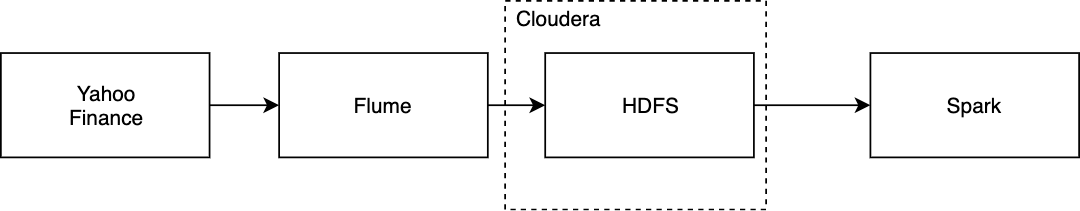
\includegraphics[scale=0.50]{images/example1} 
    \centering
    \caption{Simplified architecture of the academic pipeline}
\end{figure}

The pipeline we have picked from academia is the pipeline proposed in \cite{peng}.
The reported architecture in the paper is recaptured in Figure 4.1.
From the paper we know that the system was ran locally using local Cloudera instance.
Python was used with PySpark as the programming language and the pipeline ran normal machine learning models.
Although this information is not much, we can use it to make some observations on our system.

% for screenshots
\begin{figure}[ht!]
    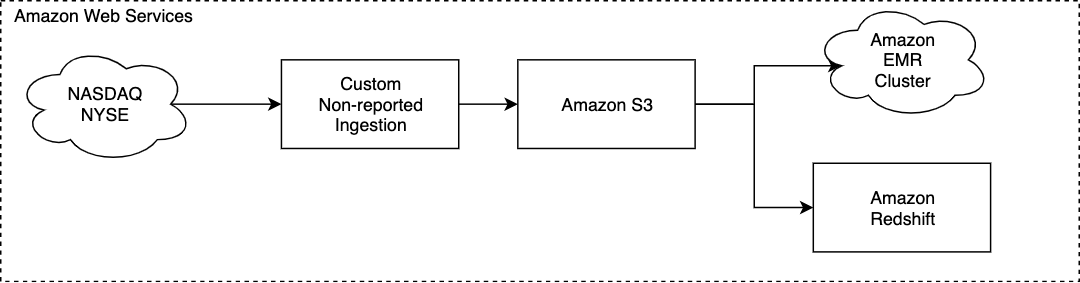
\includegraphics[scale=0.50]{images/example2} 
    \centering
    \caption{Simplified architecture of the industrial pipeline}
\end{figure}

The industrial pipeline that resembles the most of our pipeline here is the pipeline recaptured in \cite{snively}.
The high level architecture shown is presented in Figure 4.2.
What can be seen in the architecture is that we do not know much about the parts of programs that analyse the data.
Amazon EMR can be used to run almost many different big data frameworks but given that they report using it to analyse data it is higly likely that they are running multiple Spark clusters there.
But what we do know for sure is that the system is run on Amazon Web Services in large scale and we can use this to analyse our own system from the perpectives that we listed above.


We will also be quickly reflecting on the reported challenges.
We will question whetever these are significant in the sense that they could happen to any novice data scientist and is the cause of these challenges in this methology or could they have been avoided using other methods.
%We will be also analysing whetever these challenges could have been avoided and what was the root cause of these challenges.

This concludes our chapter on the proposed methology and its planned usage in the empirical part of this thesis.% were we examined and reasoned the plans we have for the empirical part of this thesis.
In the next chapter we will report the process of the implementation this in the depicted special case and see what kind of challenges were faced during it.


%After the we have the implemented pipeline, we need some ways to measure whetever our system fulfills the requirements it has been given and how does it compare with other software that might be as good as it.
%In this section we will introduce the measurements that we will be using in the chapter 6 after the implementation.
%Some of these are quantative such as the performance metrics, but these usually give very shallow view on the system.
%Because of this we will be using more qualitive methods in order to grasp the actual benefits of the pipeline.

%Our focus with the qualitive metrics is going to be on how easy the pipeline is to develop onto and how well the user can monitor changes in the pipeline.
%These are usually important factors when continuously developing a system and can affect greatly when new developers are choosing what pipelines to use.
%This also includes how automated the processes in the pipeline are and does developing and deploying the software require excessive amount of manual work.

%Some quantative metrics are taken in order to asses the fitness of the pipeline for any kind of development where it is important that iterations of the software can be swiftly build and that the whole service can run comfortably on the developers machine.
%Namely for these reasons we will examine the memory consumption of these services on a normal developing machine.
%Other quantative statistics that we can examine are processor usage, network usage and disk usage which, although not as restricting as the memory usage, can tell a lot about the performance of the system.
%For these metrics, we will be using Dockers native tools, and especially the command 'docker stats', to measure the containers usage of resources.

%As there will be a bit different pipelines with different technologies, we can get results that can be used to compare components with one another.
%This would give the reader better information and alternatives on what technologies should they could choose for their own project.
%Now we move on to the implementation chapter where we examine more closely what was done during this thesis.

% TODO: MOVE

%For this thesis we have chosen to use data from IEX API which was an open API until 30.09.2019 when the company decided to close this in order to capitalize with the closed API which free plan is in the table.
%This data is from the 5 year interval between 2014 and 2019 and the relevant values that it contains are opening prices, closing prices, highest prices, lowest prices and volumes.
%In order to test freely with this data, we will implement a simple server that serves this data into our pipeline.
